\section{Principal components}
\frame{\sectionpage}

\begin{frame}[fragile]{Principal Components}
  \begin{itemize}
  \item Have measurements on (possibly large) number of variables on some individuals.
  \item Question: can we describe data using fewer variables (because original variables correlated in some way)?
  \item Look for direction (linear combination of original variables) in which values {\em most spread out}. This is {\em first principal component}.
  \item Second principal component then direction uncorrelated with this in which values then most spread out. And so on.
  \item See whether small number of principal components captures most of variation in data.
  \item Might try to interpret principal components.
  \item If 2 components good, can make plot of data.
  \item (Like discriminant analysis, but no groups.)
  \item ``What are important ways that these data vary?''
\end{itemize}

\end{frame}

\begin{frame}[fragile]{The usual}
  
\begin{knitrout}
\definecolor{shadecolor}{rgb}{0.969, 0.969, 0.969}\color{fgcolor}\begin{kframe}
\begin{alltt}
\hlkwd{library}\hlstd{(tidyverse)}
\end{alltt}


{\ttfamily\noindent\itshape\color{messagecolor}{\#\# Loading tidyverse: ggplot2\\\#\# Loading tidyverse: tibble\\\#\# Loading tidyverse: tidyr\\\#\# Loading tidyverse: readr\\\#\# Loading tidyverse: purrr\\\#\# Loading tidyverse: dplyr}}

{\ttfamily\noindent\itshape\color{messagecolor}{\#\# Conflicts with tidy packages ----------------------------------------------}}

{\ttfamily\noindent\itshape\color{messagecolor}{\#\# filter(): dplyr, stats\\\#\# lag():\ \ \ \ dplyr, stats}}\begin{alltt}
\hlkwd{library}\hlstd{(ggrepel)}
\hlkwd{library}\hlstd{(ggbiplot)}
\end{alltt}


{\ttfamily\noindent\itshape\color{messagecolor}{\#\# Loading required package: plyr}}

{\ttfamily\noindent\itshape\color{messagecolor}{\#\# -------------------------------------------------------------------------}}

{\ttfamily\noindent\itshape\color{messagecolor}{\#\# You have loaded plyr after dplyr - this is likely to cause problems.\\\#\# If you need functions from both plyr and dplyr, please load plyr first, then dplyr:\\\#\# library(plyr); library(dplyr)}}

{\ttfamily\noindent\itshape\color{messagecolor}{\#\# -------------------------------------------------------------------------}}

{\ttfamily\noindent\itshape\color{messagecolor}{\#\# \\\#\# Attaching package: 'plyr'}}

{\ttfamily\noindent\itshape\color{messagecolor}{\#\# The following objects are masked from 'package:dplyr':\\\#\# \\\#\#\ \ \ \  arrange, count, desc, failwith, id, mutate, rename, summarise,\\\#\#\ \ \ \  summarize}}

{\ttfamily\noindent\itshape\color{messagecolor}{\#\# The following object is masked from 'package:purrr':\\\#\# \\\#\#\ \ \ \  compact}}

{\ttfamily\noindent\itshape\color{messagecolor}{\#\# Loading required package: scales}}

{\ttfamily\noindent\itshape\color{messagecolor}{\#\# \\\#\# Attaching package: 'scales'}}

{\ttfamily\noindent\itshape\color{messagecolor}{\#\# The following object is masked from 'package:purrr':\\\#\# \\\#\#\ \ \ \  discard}}

{\ttfamily\noindent\itshape\color{messagecolor}{\#\# The following objects are masked from 'package:readr':\\\#\# \\\#\#\ \ \ \  col\_factor, col\_numeric}}

{\ttfamily\noindent\itshape\color{messagecolor}{\#\# Loading required package: grid}}\end{kframe}
\end{knitrout}
  
\end{frame}

\begin{frame}[fragile]{Installing \texttt{ggbiplot}}
  
  \begin{itemize}
  \item \texttt{ggbiplot} not on CRAN, so usual
    \texttt{install.packages} will not work.
  \item Install package \texttt{devtools} first (once):
    
\begin{knitrout}
\definecolor{shadecolor}{rgb}{0.969, 0.969, 0.969}\color{fgcolor}\begin{kframe}
\begin{alltt}
\hlkwd{install.packages}\hlstd{(}\hlstr{"devtools"}\hlstd{)}
\end{alltt}
\end{kframe}
\end{knitrout}
  \item Then install \texttt{ggbiplot} (once):
\begin{knitrout}
\definecolor{shadecolor}{rgb}{0.969, 0.969, 0.969}\color{fgcolor}\begin{kframe}
\begin{alltt}
\hlkwd{library}\hlstd{(devtools)}
\hlkwd{install_github}\hlstd{(}\hlstr{"vqv/ggbiplot"}\hlstd{)}
\end{alltt}
\end{kframe}
\end{knitrout}
  \end{itemize}
  
\end{frame}

\begin{frame}[fragile]{Small example: 2 test scores for 8 people}

\begin{knitrout}
\definecolor{shadecolor}{rgb}{0.969, 0.969, 0.969}\color{fgcolor}\begin{kframe}
\begin{alltt}
\hlstd{test12}\hlkwb{=}\hlkwd{read.table}\hlstd{(}\hlstr{"test12.txt"}\hlstd{,}\hlkwc{header}\hlstd{=T)}
\hlstd{test12}
\end{alltt}
\begin{verbatim}
##   first second id
## 1     2      9  A
## 2    16     40  B
## 3     8     17  C
## 4    18     43  D
## 5    10     25  E
## 6     4     10  F
## 7    10     27  G
## 8    12     30  H
\end{verbatim}
\end{kframe}
\end{knitrout}

\begin{knitrout}
\definecolor{shadecolor}{rgb}{0.969, 0.969, 0.969}\color{fgcolor}\begin{kframe}
\begin{alltt}
\hlstd{g}\hlkwb{=}\hlkwd{ggplot}\hlstd{(test12,}\hlkwd{aes}\hlstd{(}\hlkwc{x}\hlstd{=first,}\hlkwc{y}\hlstd{=second,}\hlkwc{label}\hlstd{=id))}\hlopt{+}
  \hlkwd{geom_point}\hlstd{()}\hlopt{+}\hlkwd{geom_text_repel}\hlstd{()}
\end{alltt}
\end{kframe}
\end{knitrout}
    
\end{frame}

\begin{frame}[fragile]{The plot}

\begin{knitrout}
\definecolor{shadecolor}{rgb}{0.969, 0.969, 0.969}\color{fgcolor}\begin{kframe}
\begin{alltt}
\hlstd{g}
\end{alltt}
\end{kframe}
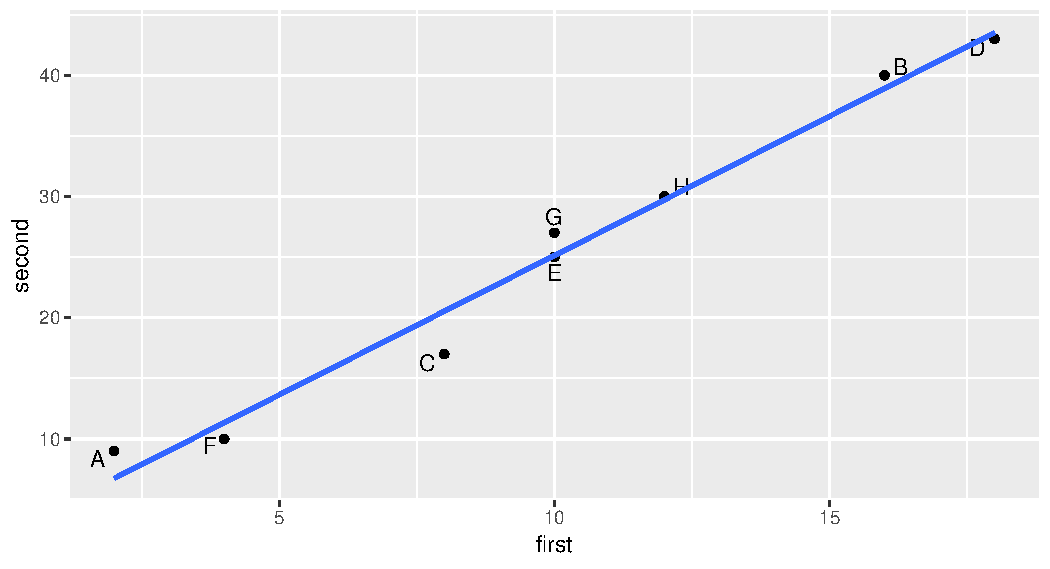
\includegraphics[width=\maxwidth]{figure/ff2-1} 

\end{knitrout}
  
%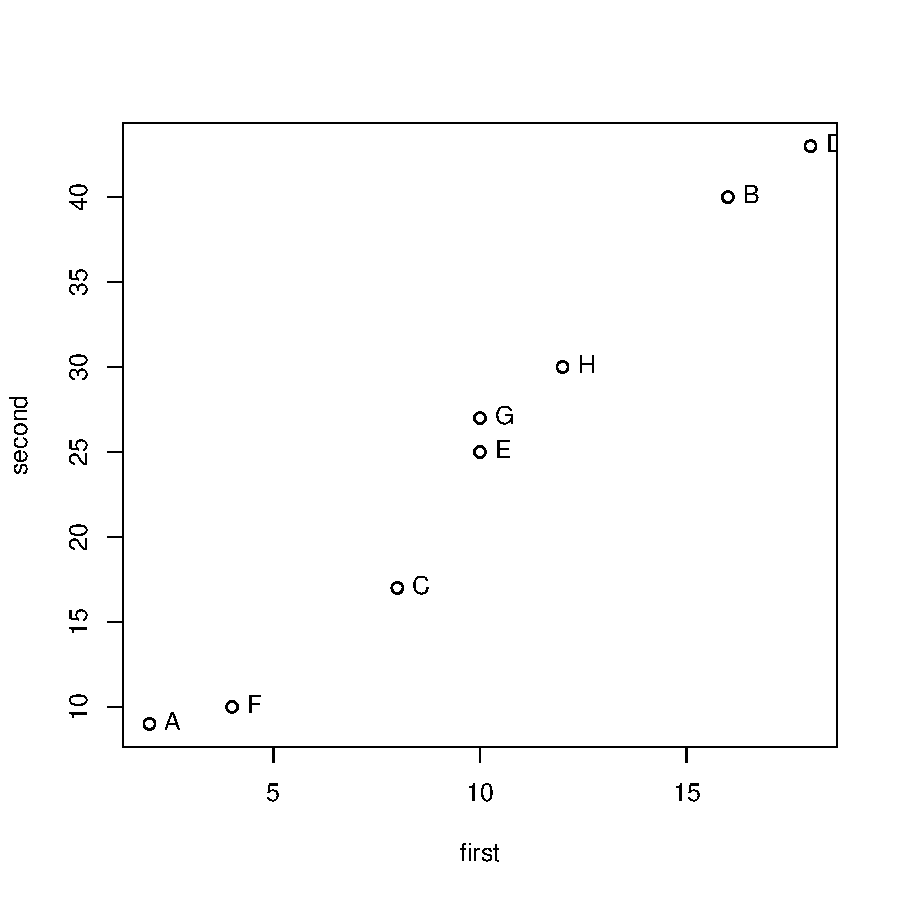
\includegraphics[height=\textheight]{bPrincomp-testt}  
  
\end{frame}

\begin{frame}[fragile]{Principal component analysis}

Strongly correlated, so data nearly 1-dimensional. 

\begin{knitrout}
\definecolor{shadecolor}{rgb}{0.969, 0.969, 0.969}\color{fgcolor}\begin{kframe}
\begin{alltt}
\hlkwd{with}\hlstd{(test12,}\hlkwd{cor}\hlstd{(first,second))}
\end{alltt}
\begin{verbatim}
## [1] 0.989078
\end{verbatim}
\end{kframe}
\end{knitrout}

Make a score summarizing this one dimension. Like this:

\begin{knitrout}\small
\definecolor{shadecolor}{rgb}{0.969, 0.969, 0.969}\color{fgcolor}\begin{kframe}
\begin{alltt}
\hlstd{test12.pc}\hlkwb{=}\hlkwd{princomp}\hlstd{(test12[,}\hlnum{1}\hlopt{:}\hlnum{2}\hlstd{],}\hlkwc{cor}\hlstd{=T)}
\hlkwd{summary}\hlstd{(test12.pc)}
\end{alltt}
\begin{verbatim}
## Importance of components:
##                          Comp.1      Comp.2
## Standard deviation     1.410347 0.104508582
## Proportion of Variance 0.994539 0.005461022
## Cumulative Proportion  0.994539 1.000000000
\end{verbatim}
\end{kframe}
\end{knitrout}

\begin{itemize}
\item ``Standard deviation'' shows relative importance of components
  (as for LDs in discriminant analysis)
\item Here, first one explains almost all (99.4\%) of variability.
\end{itemize}
  
\end{frame}

\begin{frame}[fragile]{Scree plot}
  
\begin{knitrout}
\definecolor{shadecolor}{rgb}{0.969, 0.969, 0.969}\color{fgcolor}\begin{kframe}
\begin{alltt}
\hlkwd{ggscreeplot}\hlstd{(test12.pc)}
\end{alltt}
\end{kframe}
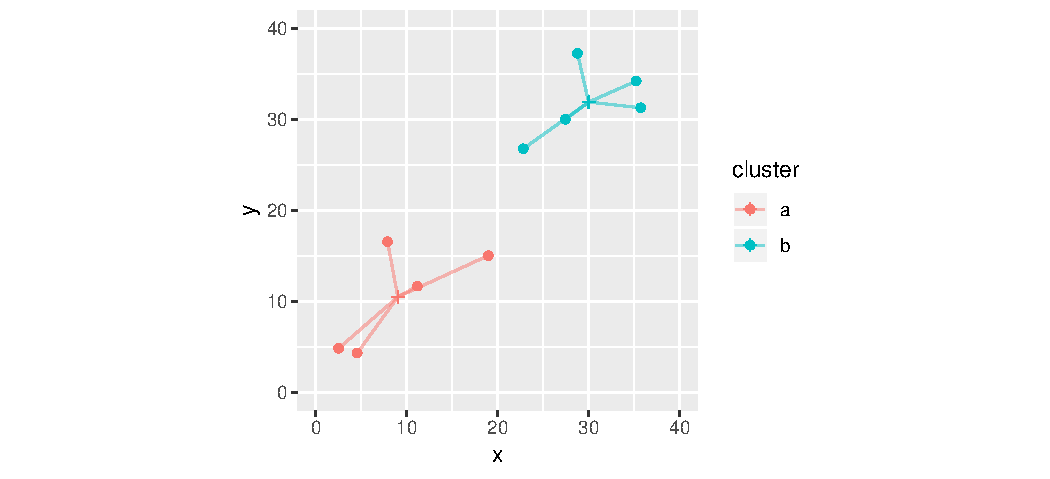
\includegraphics[width=\maxwidth]{figure/unnamed-chunk-5-1} 

\end{knitrout}
  
\end{frame}


\begin{frame}[fragile]{Component loadings}
  
  explain how each principal component depends on (standardized)
  original variables (test scores):
  
\begin{knitrout}
\definecolor{shadecolor}{rgb}{0.969, 0.969, 0.969}\color{fgcolor}\begin{kframe}
\begin{alltt}
\hlstd{test12.pc}\hlopt{$}\hlstd{loadings}
\end{alltt}
\begin{verbatim}
## 
## Loadings:
##        Comp.1 Comp.2
## first  -0.707  0.707
## second -0.707 -0.707
## 
##                Comp.1 Comp.2
## SS loadings       1.0    1.0
## Proportion Var    0.5    0.5
## Cumulative Var    0.5    1.0
\end{verbatim}
\end{kframe}
\end{knitrout}

First component basically negative sum of (standardized) test
scores. That is, person tends to score similarly on two tests, and a
composite score would summarize performance.
  
\end{frame}

\begin{frame}[fragile]{Component scores}

\begin{knitrout}
\definecolor{shadecolor}{rgb}{0.969, 0.969, 0.969}\color{fgcolor}\begin{kframe}
\begin{alltt}
\hlstd{d}\hlkwb{=}\hlkwd{data.frame}\hlstd{(test12,test12.pc}\hlopt{$}\hlstd{scores) ; d}
\end{alltt}
\begin{verbatim}
##   first second id       Comp.1       Comp.2
## 1     2      9  A  2.071819003 -0.146981782
## 2    16     40  B -1.719862811 -0.055762223
## 3     8     17  C  0.762289708  0.207589512
## 4    18     43  D -2.176267535  0.042533250
## 5    10     25  E  0.007460609  0.007460609
## 6     4     10  F  1.734784030  0.070683441
## 7    10     27  G -0.111909141 -0.111909141
## 8    12     30  H -0.568313864 -0.013613668
\end{verbatim}
\end{kframe}
\end{knitrout}
%$

\begin{itemize}
\item Person A is a low scorer, high positive \texttt{comp.1} score.
\item Person D is high scorer, high negative \texttt{comp.1} score.
\item Person E average scorer, near-zero \texttt{comp.1} score.
\item \texttt{comp.2} says basically nothing.
\end{itemize}

\end{frame}

\begin{frame}[fragile]{Plot of scores}

\begin{knitrout}
\definecolor{shadecolor}{rgb}{0.969, 0.969, 0.969}\color{fgcolor}\begin{kframe}
\begin{alltt}
\hlkwd{ggplot}\hlstd{(d,}\hlkwd{aes}\hlstd{(}\hlkwc{x}\hlstd{=Comp.1,}\hlkwc{y}\hlstd{=Comp.2,}\hlkwc{label}\hlstd{=id))}\hlopt{+}\hlkwd{geom_point}\hlstd{()}\hlopt{+}
  \hlkwd{geom_text_repel}\hlstd{()}
\end{alltt}
\end{kframe}
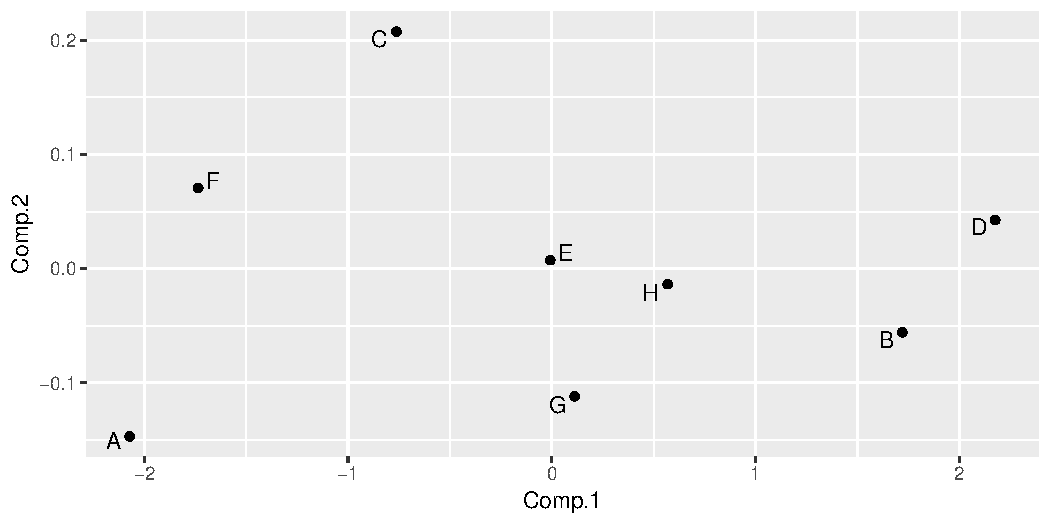
\includegraphics[width=\maxwidth]{figure/score-plot-1} 

\end{knitrout}

  
%  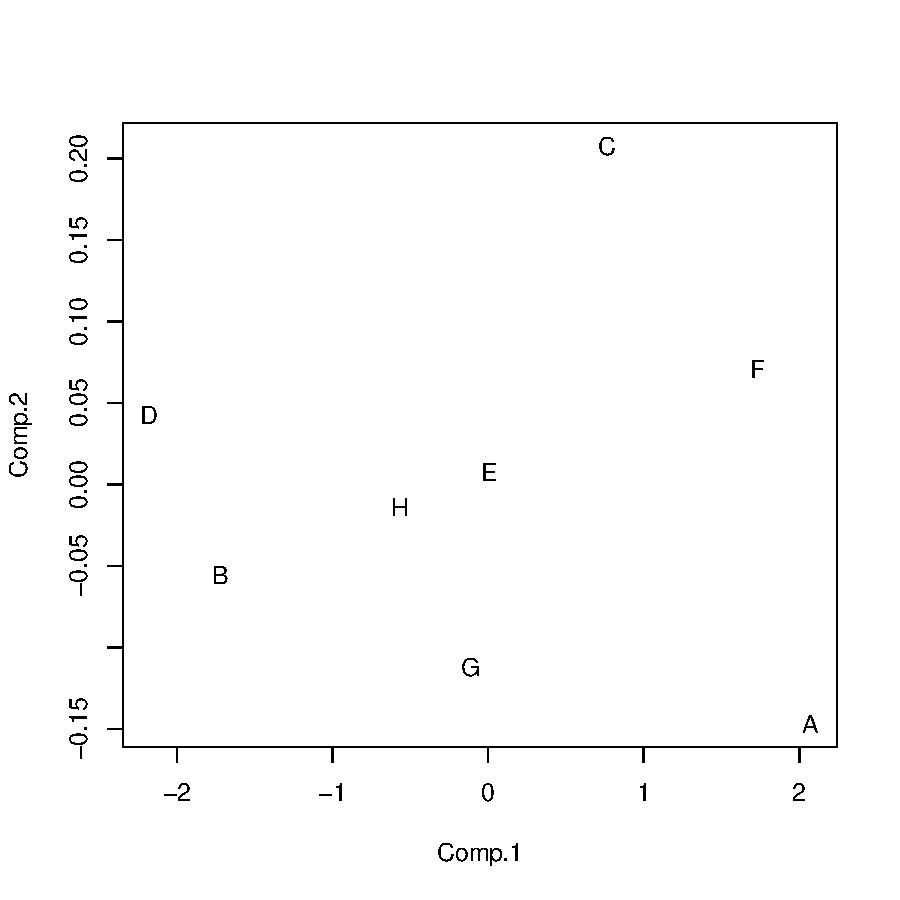
\includegraphics[height=\textheight]{bPrincomp-score-plot}
  
\end{frame}

\begin{frame}[fragile]{Comments}
  
  \begin{itemize}
  \item Vertical scale exaggerates importance of \texttt{comp.2}.
    \item Fix up to get axes on same scale:
\begin{knitrout}
\definecolor{shadecolor}{rgb}{0.969, 0.969, 0.969}\color{fgcolor}\begin{kframe}
\begin{alltt}
\hlstd{g}\hlkwb{=}\hlkwd{ggplot}\hlstd{(d,}\hlkwd{aes}\hlstd{(}\hlkwc{x}\hlstd{=Comp.1,}\hlkwc{y}\hlstd{=Comp.2,}\hlkwc{label}\hlstd{=id))}\hlopt{+}
  \hlkwd{geom_point}\hlstd{()}\hlopt{+}\hlkwd{geom_text_repel}\hlstd{()}\hlopt{+}
  \hlkwd{coord_fixed}\hlstd{()}
\end{alltt}
\end{kframe}
\end{knitrout}
\item Shows how exam scores really spread out along one dimension:

\begin{knitrout}
\definecolor{shadecolor}{rgb}{0.969, 0.969, 0.969}\color{fgcolor}\begin{kframe}
\begin{alltt}
\hlstd{g}
\end{alltt}
\end{kframe}
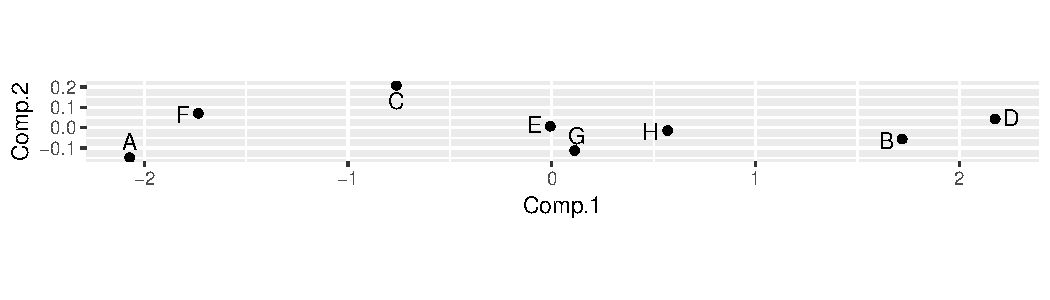
\includegraphics[width=\maxwidth]{figure/eqsc2-1} 

\end{knitrout}
  
  \end{itemize}

\end{frame}


\begin{frame}[fragile]{The biplot}
  
  \begin{itemize}
  \item Plotting variables and individuals on one plot.
  \item Shows how components and original variables related.
  \item Shows how individuals score on each component, and therefore
    suggests how they score on each variable.
  \item Add \texttt{labels} option to identify individuals:
    
\begin{knitrout}
\definecolor{shadecolor}{rgb}{0.969, 0.969, 0.969}\color{fgcolor}\begin{kframe}
\begin{alltt}
\hlstd{g}\hlkwb{=}\hlkwd{ggbiplot}\hlstd{(test12.pc,}\hlkwc{labels}\hlstd{=test12}\hlopt{$}\hlstd{id)}
\end{alltt}
\end{kframe}
\end{knitrout}
    
  \end{itemize}
  
\end{frame}

\begin{frame}[fragile]{The biplot}
  
\begin{knitrout}
\definecolor{shadecolor}{rgb}{0.969, 0.969, 0.969}\color{fgcolor}
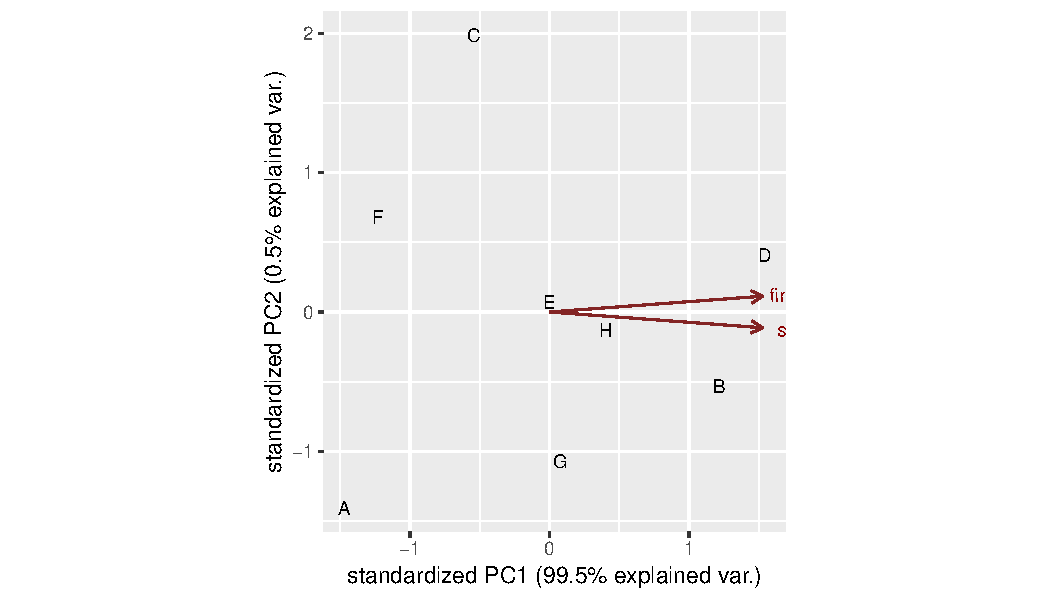
\includegraphics[width=\maxwidth]{figure/ff3-1} 

\end{knitrout}
  
  
%  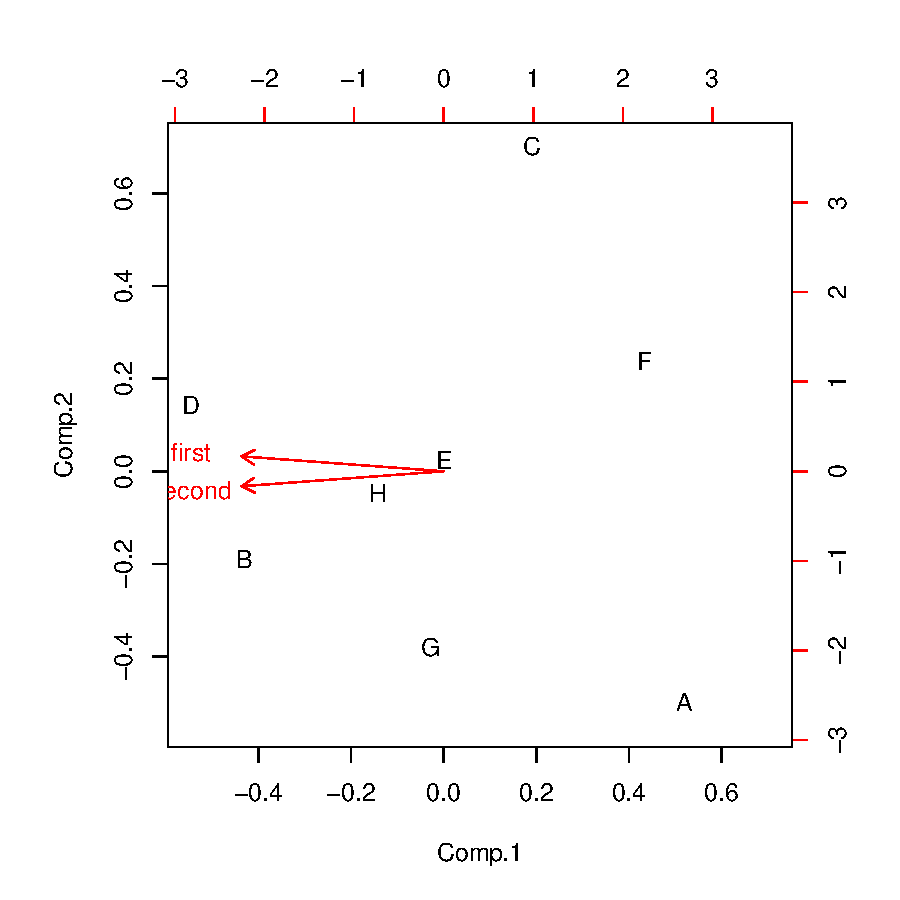
\includegraphics[height=\textheight]{bPrincomp-test-biplot}
  
\end{frame}

\begin{frame}[fragile]{Comments}
  
  \begin{itemize}
  \item Variables point almost same direction (left). Thus very
    negative value on \texttt{comp.1} goes with high scores on both
    tests, and test scores highly correlated.
  \item Position of individuals on plot according to scores on
    principal components, implies values on original variables. Eg.:
    \begin{itemize}
    \item D very negative on \texttt{comp.1}, high scorer on both tests.
    \item A and F very positive on \texttt{comp.1}, poor scorers on
      both tests.
    \item C positive on \texttt{comp.2}, high score on first
      test relative to second.
    \item A negative on \texttt{comp.2}, high score on second test
      relative to first.
    \end{itemize}
  \end{itemize}
  
\end{frame}


\begin{frame}[fragile]{Track running data}

  Maybe another example? eg. football stats (NFL or college?)
  
(1984) track running records for distances 100m to marathon, arranged by country. Countries labelled by (mostly) Internet domain names:

{\footnotesize
\begin{knitrout}
\definecolor{shadecolor}{rgb}{0.969, 0.969, 0.969}\color{fgcolor}\begin{kframe}
\begin{alltt}
\hlstd{track}\hlkwb{=}\hlkwd{read.table}\hlstd{(}\hlstr{"men_track_field.txt"}\hlstd{,}\hlkwc{header}\hlstd{=T)}
\hlstd{track[}\hlkwd{c}\hlstd{(}\hlnum{1}\hlopt{:}\hlnum{8}\hlstd{,}\hlnum{52}\hlopt{:}\hlnum{55}\hlstd{),]}
\end{alltt}
\begin{verbatim}
##     m100  m200  m400 m800 m1500 m5000 m10000 marathon country
## 1  10.39 20.81 46.84 1.81  3.70 14.04  29.36   137.72      ar
## 2  10.31 20.06 44.84 1.74  3.57 13.28  27.66   128.30      au
## 3  10.44 20.81 46.82 1.79  3.60 13.26  27.72   135.90      at
## 4  10.34 20.68 45.04 1.73  3.60 13.22  27.45   129.95      be
## 5  10.28 20.58 45.91 1.80  3.75 14.68  30.55   146.62      bm
## 6  10.22 20.43 45.21 1.73  3.66 13.62  28.62   133.13      br
## 7  10.64 21.52 48.30 1.80  3.85 14.45  30.28   139.95      bu
## 8  10.17 20.22 45.68 1.76  3.63 13.55  28.09   130.15      ca
## 52 10.71 21.43 47.60 1.79  3.67 13.56  28.58   131.50      tr
## 53  9.93 19.75 43.86 1.73  3.53 13.20  27.43   128.22      us
## 54 10.07 20.00 44.60 1.75  3.59 13.20  27.53   130.55      ru
## 55 10.82 21.86 49.00 2.02  4.24 16.28  34.71   161.83      ws
\end{verbatim}
\end{kframe}
\end{knitrout}
}
  
\end{frame}

\begin{frame}[fragile]{Data and aims}

  \begin{itemize}
  \item 
Times in seconds 100m-400m, in minutes for rest (800m, 1500m, 5000m, 10000m, marathon).
\item This taken care of by standardization.
\item 8 variables; can we summarize by fewer and gain some insight?
\item In particular, if 2 components tell most of story, what do we see in a plot?

  \end{itemize}

  
\end{frame}


\begin{frame}[fragile]{Fit and examine principal components}
 

  
{\small  
\begin{knitrout}
\definecolor{shadecolor}{rgb}{0.969, 0.969, 0.969}\color{fgcolor}\begin{kframe}
\begin{alltt}
\hlstd{track.pc}\hlkwb{=}\hlkwd{princomp}\hlstd{(track[,}\hlnum{1}\hlopt{:}\hlnum{8}\hlstd{],}\hlkwc{cor}\hlstd{=T)}
\hlkwd{summary}\hlstd{(track.pc)}
\end{alltt}
\begin{verbatim}
## Importance of components:
##                           Comp.1    Comp.2
## Standard deviation     2.5733531 0.9368128
## Proportion of Variance 0.8277683 0.1097023
## Cumulative Proportion  0.8277683 0.9374706
##                            Comp.3     Comp.4
## Standard deviation     0.39915052 0.35220645
## Proportion of Variance 0.01991514 0.01550617
## Cumulative Proportion  0.95738570 0.97289187
##                             Comp.5      Comp.6
## Standard deviation     0.282630981 0.260701267
## Proportion of Variance 0.009985034 0.008495644
## Cumulative Proportion  0.982876903 0.991372547
##                             Comp.7      Comp.8
## Standard deviation     0.215451919 0.150333291
## Proportion of Variance 0.005802441 0.002825012
## Cumulative Proportion  0.997174988 1.000000000
\end{verbatim}
\end{kframe}
\end{knitrout}
}

\end{frame}



  
  


\begin{frame}[fragile]{Scree plot}

\begin{knitrout}
\definecolor{shadecolor}{rgb}{0.969, 0.969, 0.969}\color{fgcolor}\begin{kframe}
\begin{alltt}
\hlkwd{ggscreeplot}\hlstd{(track.pc)}
\end{alltt}
\end{kframe}
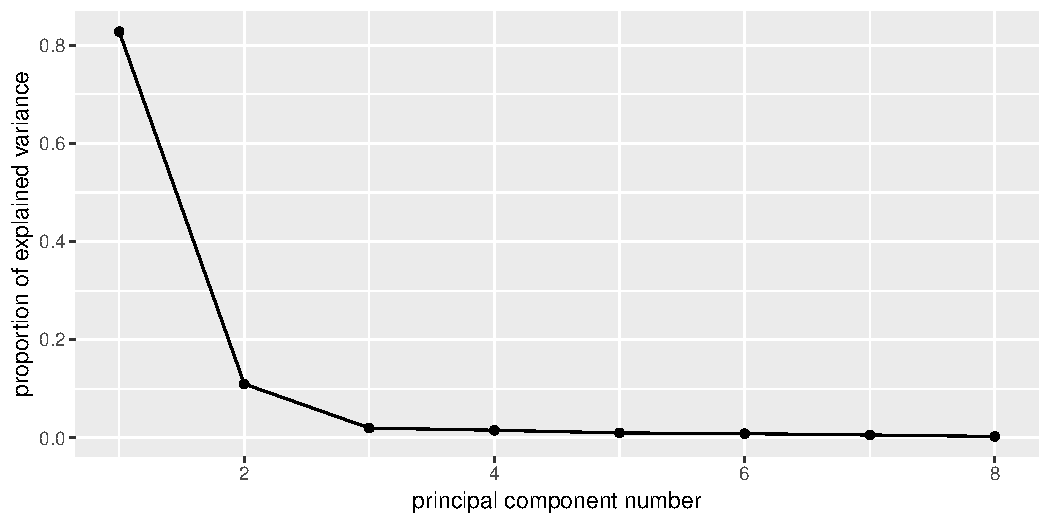
\includegraphics[width=\maxwidth]{figure/scree-b-1} 

\end{knitrout}

\end{frame}


\begin{frame}[fragile]{How many components?}
  
  \begin{itemize}
  \item As for discriminant analysis, look for ``elbow'' in scree plot.
  \item See one here at 3 components; everything 3 and beyond is ``scree''.
  \item So take 2 components.
  \item Note difference from discriminant analysis: want ``large''
    rather than ``small'', so go 1 step left of elbow.
  \item Another criterion: any component with eigenvalue bigger than
    about 1 is worth including. 2nd one here has eigenvalue just less
    than 1.
  \item Refer back to \texttt{summary}: cumulative proportion of
    variance explained for 2 components is 93.7\%, pleasantly high. 2
    components tell almost whole story.
  \end{itemize}
  
\end{frame}

\begin{frame}[fragile]{How do components depend on original variables?}
  
  Loadings:

\begin{knitrout}
\definecolor{shadecolor}{rgb}{0.969, 0.969, 0.969}\color{fgcolor}\begin{kframe}
\begin{alltt}
\hlstd{track.pc}\hlopt{$}\hlstd{loadings[,}\hlnum{1}\hlopt{:}\hlnum{4}\hlstd{]}
\end{alltt}
\begin{verbatim}
##              Comp.1      Comp.2     Comp.3      Comp.4
## m100     -0.3175565 -0.56687750  0.3322620 -0.12762827
## m200     -0.3369792 -0.46162589  0.3606567  0.25911576
## m400     -0.3556454 -0.24827331 -0.5604674 -0.65234077
## m800     -0.3686841 -0.01242993 -0.5324823  0.47999895
## m1500    -0.3728099  0.13979665 -0.1534427  0.40451039
## m5000    -0.3643741  0.31203045  0.1897643 -0.02958755
## m10000   -0.3667726  0.30685985  0.1817517 -0.08006862
## marathon -0.3419261  0.43896267  0.2632087 -0.29951213
\end{verbatim}
\end{kframe}
\end{knitrout}

  
\end{frame}

\begin{frame}[fragile]{Comments}
  
  \begin{itemize}
  \item \texttt{comp.1} loads about equally (has equal weight) on
    times over all distances.
  \item \texttt{comp.2} has large positive loading for long
    distances, large negative for short ones.
  \item \texttt{comp.3}: large negative for middle distance, large
    positive especially for short distances.
  \item Country overall good at running will have lower than average record
    times at all distances, so \texttt{comp.1}
    \emph{large}. Conversely, for countries bad at running,
    \texttt{comp.1} very negative.
  \item Countries relatively better at sprinting (low times) will be
    \emph{positive} on \texttt{comp.2}; countries relatively better at
    distance running \emph{negative} on \texttt{comp.2}.
  \end{itemize}
  
\end{frame}

\begin{frame}[fragile]{Commands for plots}
  
  \begin{itemize}
  \item Principal component scores (first two). Recall 9th column of
    data was country name abbrevs.
    
\begin{knitrout}
\definecolor{shadecolor}{rgb}{0.969, 0.969, 0.969}\color{fgcolor}\begin{kframe}
\begin{alltt}
\hlkwd{plot}\hlstd{(track.pc}\hlopt{$}\hlstd{scores[,}\hlnum{1}\hlopt{:}\hlnum{2}\hlstd{],}\hlkwc{type}\hlstd{=}\hlstr{"n"}\hlstd{)}
\hlkwd{text}\hlstd{(track.pc}\hlopt{$}\hlstd{scores[,}\hlnum{1}\hlopt{:}\hlnum{2}\hlstd{],}\hlkwd{as.character}\hlstd{(track[,}\hlnum{9}\hlstd{]))}
\end{alltt}
\end{kframe}
\end{knitrout}

\item Biplot:
  
\begin{knitrout}
\definecolor{shadecolor}{rgb}{0.969, 0.969, 0.969}\color{fgcolor}\begin{kframe}
\begin{alltt}
\hlkwd{biplot}\hlstd{(track.pc,}\hlkwc{xlabs}\hlstd{=track[,}\hlnum{9}\hlstd{])}
\end{alltt}
\end{kframe}
\end{knitrout}
    
    
  \end{itemize}
  
\end{frame}

\begin{frame}{Principal components plot}

\begin{knitrout}
\definecolor{shadecolor}{rgb}{0.969, 0.969, 0.969}\color{fgcolor}
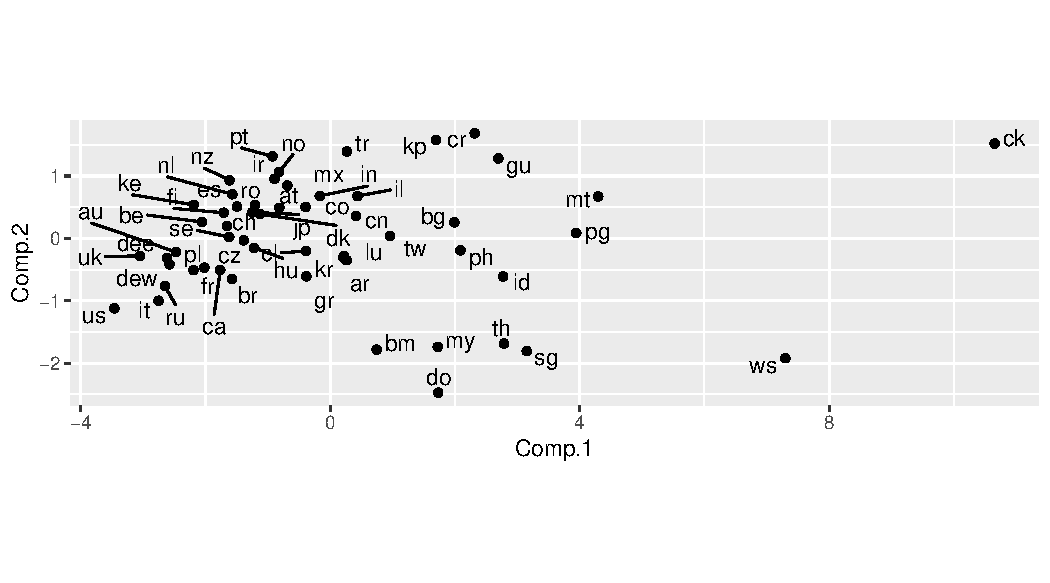
\includegraphics[width=\maxwidth]{figure/lecce-1} 

\end{knitrout}

  
\end{frame}

\begin{frame}[fragile]{Comments on principal components plot}
  
  \begin{itemize}
  \item Good running countries at right of plot: US, UK, Italy,
    Russia, East and West Germany.
  \item Bad running countries at left: Western Samoa, Cook Islands.
  \item Better sprinting countries at top: US, Italy, Russia,
    Brazil, Greece. \texttt{dr} is Dominican Republic, where sprinting
    records very good, distance records very bad.
  \item Better distance-running countries at bottom: Portugal, Norway,
    Turkey, Ireland, New Zealand, Mexico. \texttt{ke} is Kenya.
  \end{itemize}
  
\end{frame}

\begin{frame}{Biplot}

\begin{knitrout}
\definecolor{shadecolor}{rgb}{0.969, 0.969, 0.969}\color{fgcolor}
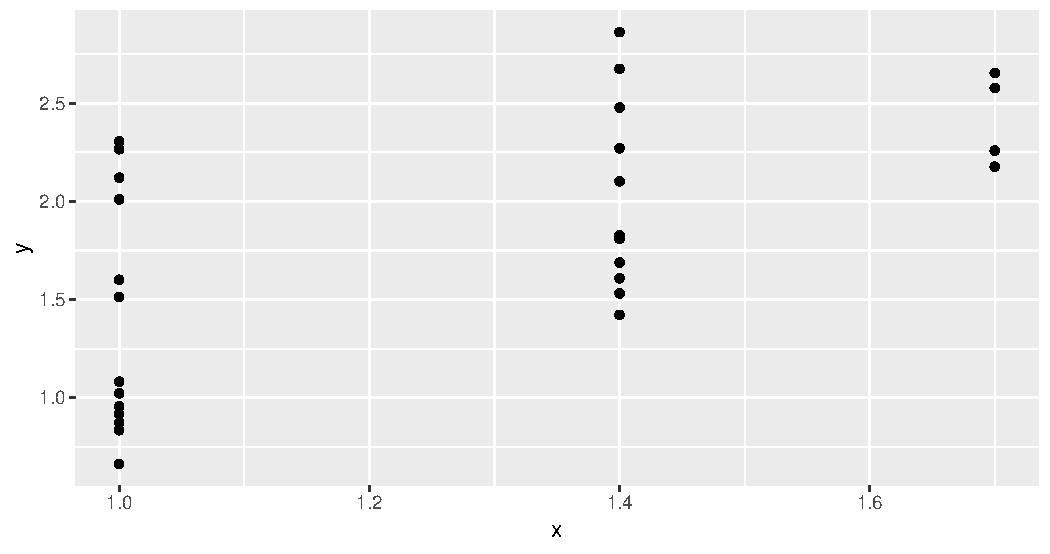
\includegraphics[width=\maxwidth]{figure/biplot2-1} 

\end{knitrout}

%  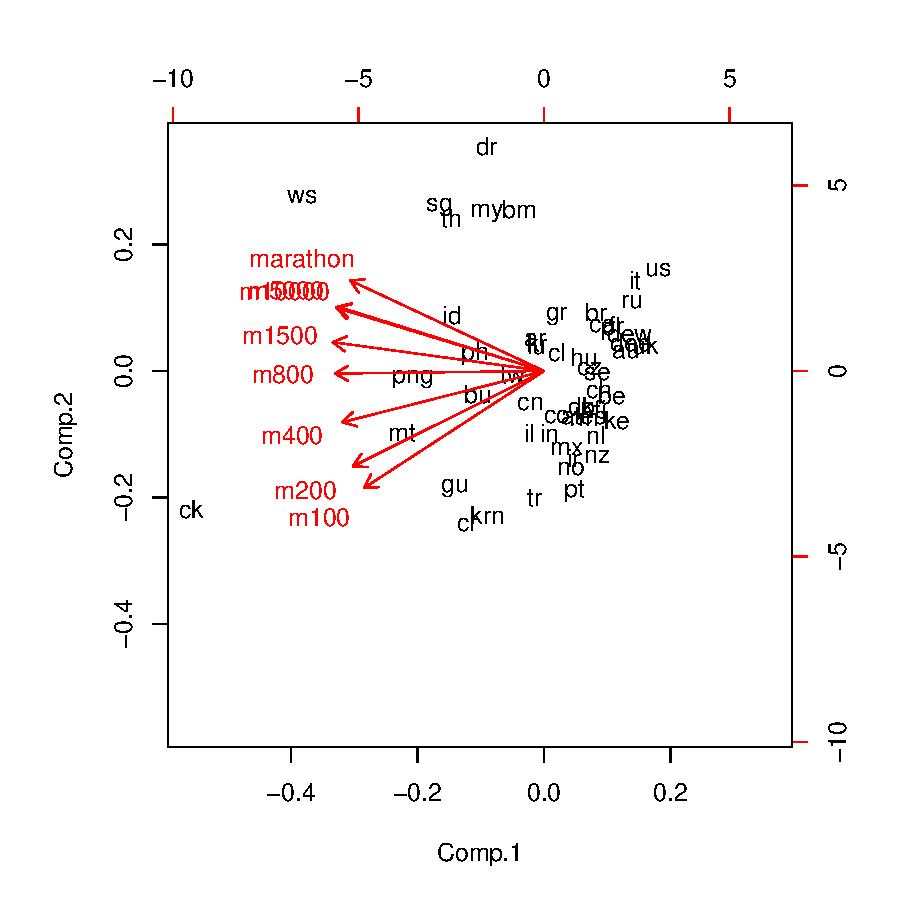
\includegraphics[height=\textheight]{bPrincomp-biplot}
  
\end{frame}

\begin{frame}{Comments on biplot}
  
  \begin{itemize}
  \item Had to do some pre-work to interpret PC plot. Biplot more self-contained.
  \item All variable arrows point left; countries on left have large
    (bad) record times overall, countries on right good overall.
  \item Variable arrows extend negatively as well. Top left = bad at
    distance running, bottom right = good at distance running.
  \item Bottom left = bad at sprinting, top right = good at
    sprinting.
  \item Doesn't require so much pre-interpretation of components.
  \end{itemize}
  
\end{frame}

\begin{frame}[fragile]{Principal components from correlation matrix}
  
  Create data file like this:

  
  \verbatiminput{cov.txt}
  
  and read in like this:
  
\begin{knitrout}
\definecolor{shadecolor}{rgb}{0.969, 0.969, 0.969}\color{fgcolor}\begin{kframe}
\begin{alltt}
\hlstd{mat}\hlkwb{=}\hlkwd{read.table}\hlstd{(}\hlstr{"cov.txt"}\hlstd{,}\hlkwc{header}\hlstd{=F)}
\hlstd{mat}
\end{alltt}
\begin{verbatim}
##        V1      V2     V3
## 1  1.0000  0.9705 -0.960
## 2  0.9705  1.0000 -0.998
## 3 -0.9600 -0.9980  1.000
\end{verbatim}
\end{kframe}
\end{knitrout}
  
\end{frame}

\begin{frame}[fragile]{Pre-processing}
  
  A little pre-processing required:
  
  \begin{itemize}
  \item Turn into matrix (from data frame)
  \item Feed into \texttt{princomp} as \texttt{covmat=}
  \end{itemize}
  
\begin{knitrout}
\definecolor{shadecolor}{rgb}{0.969, 0.969, 0.969}\color{fgcolor}\begin{kframe}
\begin{alltt}
\hlstd{matmat}\hlkwb{=}\hlkwd{as.matrix}\hlstd{(mat)}
\hlstd{mat.pc}\hlkwb{=}\hlkwd{princomp}\hlstd{(}\hlkwc{covmat}\hlstd{=matmat)}
\end{alltt}
\end{kframe}
\end{knitrout}
  
\end{frame}

\begin{frame}[fragile]{Scree plot: one component fine}

\begin{knitrout}
\definecolor{shadecolor}{rgb}{0.969, 0.969, 0.969}\color{fgcolor}\begin{kframe}
\begin{alltt}
\hlkwd{plot}\hlstd{(mat.pc,}\hlkwc{type}\hlstd{=}\hlstr{"l"}\hlstd{)}
\end{alltt}
\end{kframe}
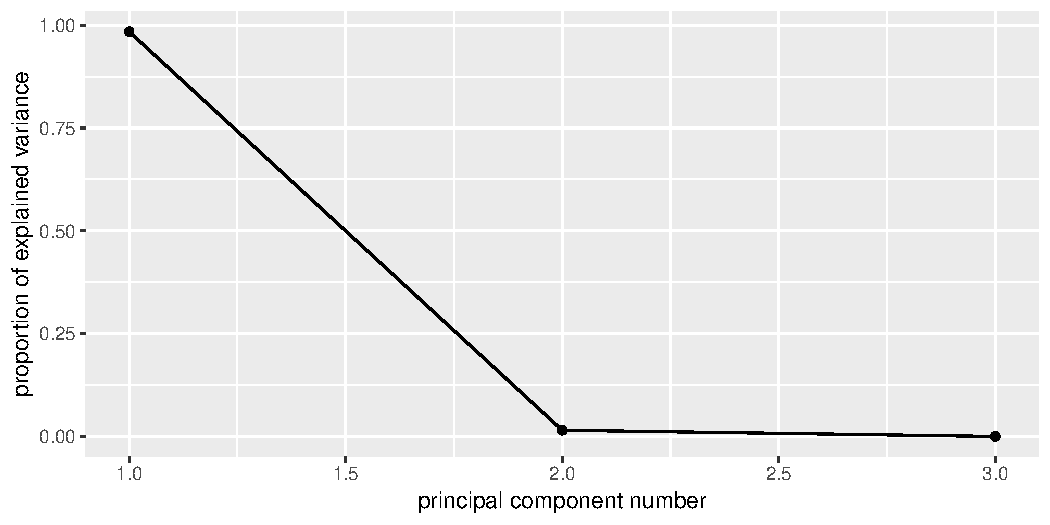
\includegraphics[width=\maxwidth]{figure/palermo-1} 

\end{knitrout}
%  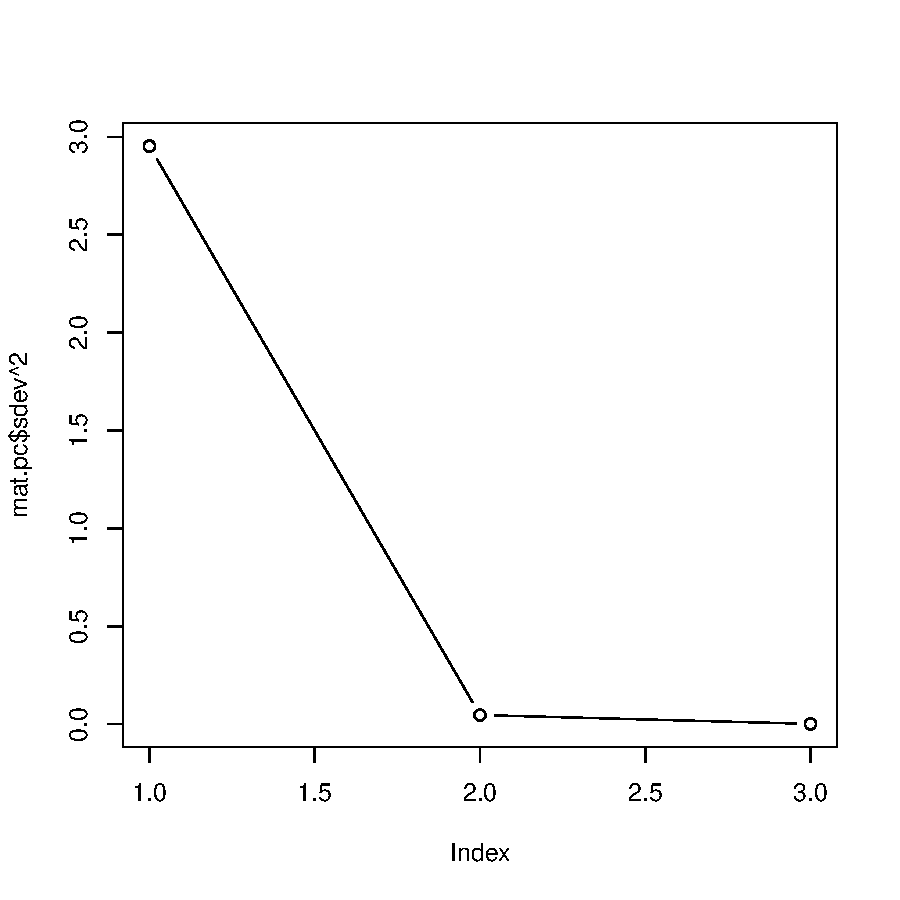
\includegraphics[height=\textheight]{bPrincomp-pc-cov}    

  
\end{frame}

\begin{frame}[fragile]{Component loadings}
  
  
  \begin{minipage}[t]{0.6\linewidth}
  Compare correlation matrix:

{\footnotesize
\begin{knitrout}
\definecolor{shadecolor}{rgb}{0.969, 0.969, 0.969}\color{fgcolor}\begin{kframe}
\begin{alltt}
\hlstd{mat}
\end{alltt}
\begin{verbatim}
##        V1      V2     V3
## 1  1.0000  0.9705 -0.960
## 2  0.9705  1.0000 -0.998
## 3 -0.9600 -0.9980  1.000
\end{verbatim}
\end{kframe}
\end{knitrout}
}

with component loadings

{\footnotesize
\begin{knitrout}
\definecolor{shadecolor}{rgb}{0.969, 0.969, 0.969}\color{fgcolor}\begin{kframe}
\begin{alltt}
\hlstd{mat.pc}\hlopt{$}\hlstd{loadings}
\end{alltt}
\begin{verbatim}
## 
## Loadings:
##    Comp.1 Comp.2 Comp.3
## V1 -0.573  0.812 -0.112
## V2 -0.581 -0.306  0.755
## V3  0.578  0.498  0.646
## 
##                Comp.1 Comp.2 Comp.3
## SS loadings     1.000  1.000  1.000
## Proportion Var  0.333  0.333  0.333
## Cumulative Var  0.333  0.667  1.000
\end{verbatim}
\end{kframe}
\end{knitrout}
}

%$
  \end{minipage}
  \begin{minipage}[t]{0.37\linewidth}
    \begin{itemize}
    \item When V1 large, V2 also large, V3 small.
    \item Then \texttt{comp.1} \emph{negative}.
    \item When V1 small, V2 small, V3 large.
    \item Then \texttt{comp.1} \emph{positive}.
      
    \end{itemize}
  \end{minipage}
\end{frame}


\begin{frame}[fragile]{No scores}
  
  \begin{itemize}
  \item With correlation matrix rather than data, no component scores
  \item So no principal component plot
  \item and no biplot. 
  \end{itemize}
  
\end{frame}
